\subsection{Sprint 3: da 2024-05-06 a 2024-05-21}
\par Dato che il \PdQ\ non ha registrato avanzamenti significativi negli \glossario{sprint} precedenti, il team ha fissato come obiettivo primario l'individuazione delle metriche di qualità. Inoltre, il gruppo ha programmato il \glossario{benchmark} dei modelli e l'implementazione delle funzionalità back-end correlate alla libreria \glossario{txtai}. Contestualmente, verrà avviato lo sviluppo della web app con \glossario{Streamlit} e verranno configurati \glossario{framework} back-end e front-end alternativi. Infine, il team ha deciso di riorganizzare la struttura del \PdP.

\subsubsection{Obiettivi}
\begin{itemize}
  \item Aggiornamento delle \NdP\ con le modalità di integrazione Jira - Github;
  \item Stesura verbali interni ed esterni;
  \item Formalizzazione delle metriche di qualità nelle \NdP;
  \item Inserimento nel \PdQ\ delle soglie di tolleranza stabilite per ciascuna metrica;
  \item Stesura delle sezioni incomplete nel documento di \AdR\ ed espansione dei casi e sottocasi d'uso;
  \item Elaborazione di una relazione sul framework Streamlit (pro e contro, confronto con alternative);
  \item Pianificazione e preventivo dello sprint 4;
  \item Miglioramento della struttura del \PdP;
  \item Creazione della prima bozza dell'interfaccia grafica;
  \item Inizio sviluppo della web app;
  \item Creazione di un doppio indice per la ricerca semantica e la generazione del prompt;
  \item Benchmark dei modelli;
  \item Configurazione di framework back-end e front-end alternativi (Flask, Django, Vue.js, Next.js).
\end{itemize}

\begin{figure}[H]
  \centering
  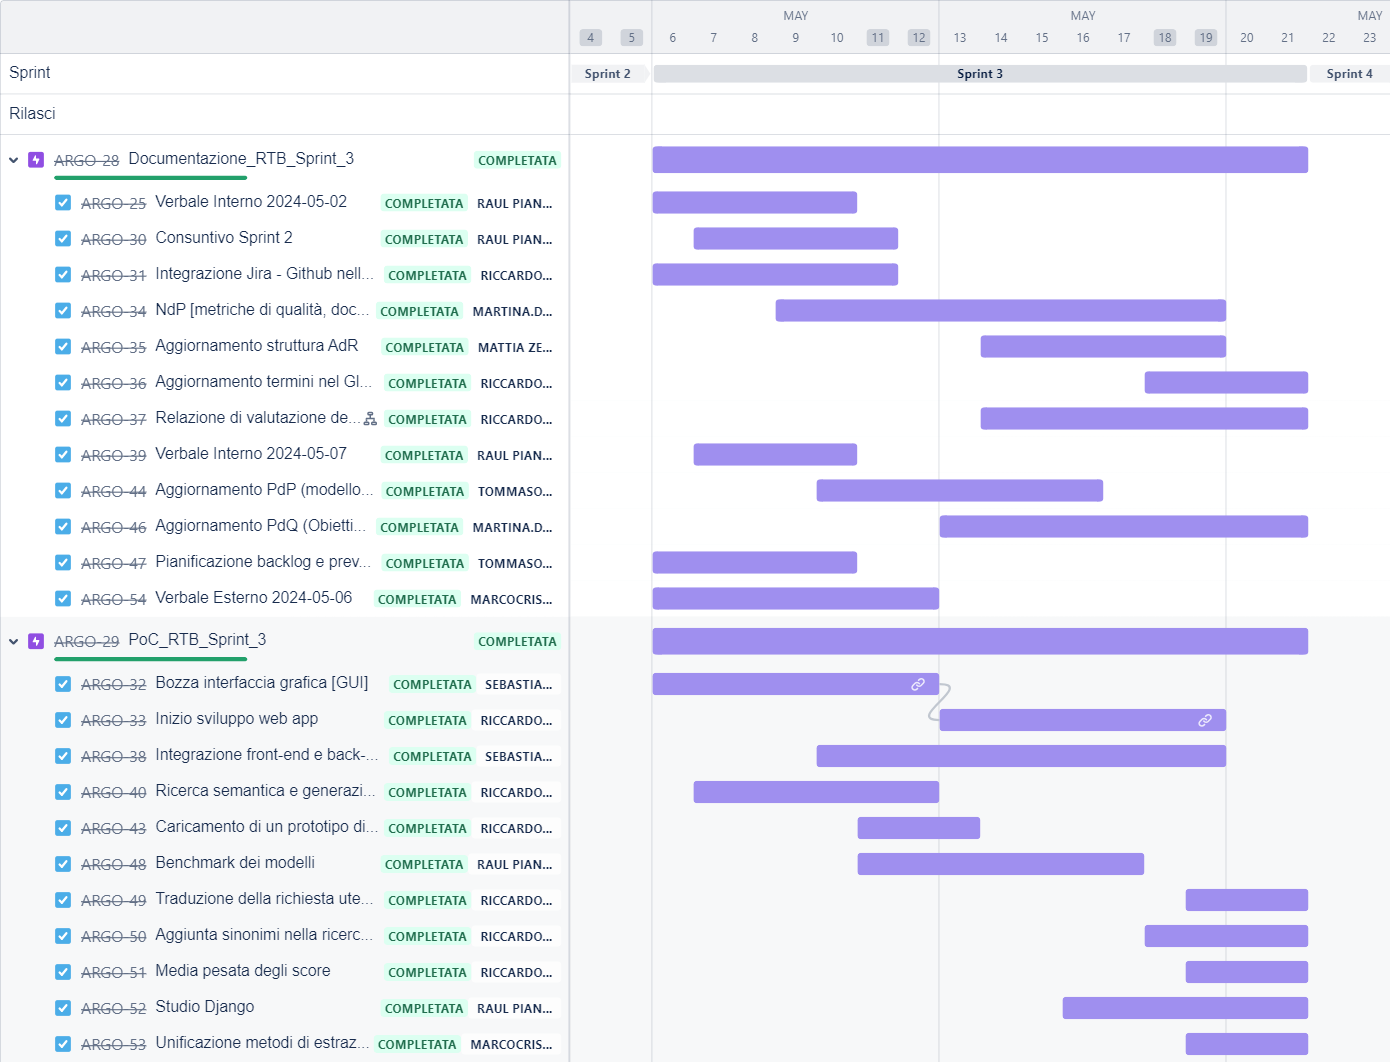
\includegraphics[width=0.90\textwidth]{assets/Pianificazione/Sprint-3/gantt.png}
  \caption{Sprint 3 - Diagramma di Gantt}\label{fig:sprint-3-gantt}
\end{figure}
